\documentclass[14pt]{article}

\def\inputGnumericTable{}  
 
\usepackage[utf8]{inputenc}
\usepackage[T1]{fontenc}
\usepackage[spanish]{babel}
\usepackage{times}
\usepackage{fancyvrb}
\usepackage{stackrel}
\usepackage{graphics,graphicx,float}
\usepackage{amsmath,amsfonts,amsthm}
\usepackage{algorithm}
\usepackage{tabularx,ragged2e,booktabs,caption}
\usepackage{subfig}
\usepackage{epstopdf}

\usepackage{multicol}
	\setlength{\columnsep}{1cm}
	
\usepackage{hyperref}
\usepackage{pmboxdraw}
\usepackage{babel}
\usepackage{multirow}
\usepackage{enumerate}

\usepackage{color}                                            
\usepackage{array}                                            
\usepackage{longtable}                                        
\usepackage{calc}                                             
\usepackage{multirow}                                         
\usepackage{hhline}                                           
\usepackage{ifthen}    

%\usepackage{fullpage}


\graphicspath{{./img/}}


\usepackage{graphicx}
\usepackage{algpseudocode}
 
\usepackage{color}
\definecolor{gray97}{gray}{.97}
\definecolor{gray75}{gray}{.75}
\definecolor{gray45}{gray}{.45}
 
\usepackage{listings}
\lstset{ frame=Ltb,
     framerule=0pt,
     aboveskip=0.5cm,
     framextopmargin=3pt,
     framexbottommargin=3pt,
     framexleftmargin=0.4cm,
     framesep=0pt,
     rulesep=.4pt,
     backgroundcolor=\color{gray97},
     rulesepcolor=\color{black},
     extendedchars=true,
     %
     stringstyle=\ttfamily,
     showstringspaces = false,
     basicstyle=\small\ttfamily,
     commentstyle=\color{gray45},
     keywordstyle=\bfseries,
     %
     numbers=left,
     numbersep=15pt,
     numberstyle=\tiny,
     numberfirstline = false,
     breaklines=true,
     tabsize=2,
   }
 
% minimizar fragmentado de listados
\lstnewenvironment{listing}[1][]
   {\lstset{#1}\pagebreak[0]}{\pagebreak[0]}
 
\lstdefinestyle{consola}
   {basicstyle=\scriptsize\bf\ttfamily,
    backgroundcolor=\color{gray75},
   }
 
\lstdefinestyle{C}
   {language=C,
   }
\lstdefinestyle{bash}
   {language=bash,
   }
   
  \renewcommand{\lstlistingname}{Algoritmo}% Listing -> Algorithm
\renewcommand{\lstlistlistingname}{Lista de \lstlistingname s}

\newcommand\tab[1][1cm]{\hspace*{#1}}

%%%%%%%%%%%%%%%%%%%%%%%%%%%%%%%%%%%%%
%%%%%%%%%%%%%%%%%%%%%%%%%%%%%%%%%%%%%

\begin{document}

\begin{titlepage}

\begin{center}
	\vspace*{-1in}
	\begin{figure}[htb]
		\begin{center}
			
\includegraphics[width=12cm]{./descarga.png}
		\end{center}
	\end{figure}
	
E.T.S. de Ingenierías Informática y de Telecomunicaciones\\
\vspace*{0.4in}
\begin{large}
Práctica 2:\\
\end{large}
\vspace*{0.2in}
\begin{huge}
\textbf{Problema del Aprendizaje de Pesos en Características (APC)}\\
\end{huge}
\vspace*{0.9in}
\begin{large}
DECSAI\\
\vspace*{0.1in}
Metaheuristicas. Grupo 1: Lunes de 17:30 a 19:30\\
\end{large}
\vspace*{0.3in}
\rule{80mm}{0.1mm}\\
\vspace*{0.1in}
\begin{large}
Autor:\\
Iván Lopez Justicia. DNI: 26514896J. 
email: ivanlopez27@correo.ugr.es
\end{large}
\end{center}
\end{titlepage}

\date{}

\newpage 

\tableofcontents
%\lstlistoflistings
\vfill

\newpage
%
\section{Descripción del problema}
El problema del Aprendizaje de Pesos en Características (APC) es un problema de búsqueda con codificación real en el espacion n-dimensional, para n características. Consiste en obtener un vector de pesos que permita ponderar las características asociadas a un dato con la intención de obtener un mejor porcentaje de clasificación de datos futuros. \\

Tenemos una muestra de datos, $X = {x_{1}, x_{2},...,x_{n}}$, en la que cada dato $x_{i}$ está formado por un conjunto de características ${c_{1}, c_{2},...,c_{n}}$, además, también contiene la clase de cada dato, al final del conjunto de características. Con estos datos, tenemos que obtener un vector $W$ de pesos ${w_{1}, w_{2},...,w_{n}}$ donde cada $w_{i}$ pondera la característica $c_{i}$ y que el vector de pesos nos permita obtener un alto porcentaje de otro conjunto de datos nuevos o desconocidos hasta la comprobación de la calidad de nuestro vector de pesos W.

En esta práctica se van a realizar dos tareas: 

\begin{enumerate}
\item Obtener el vector de pesos (aprendizaje)
\item Valorar la calidad del vector (validación).
\end{enumerate}

Para la validación vamos a utilizar la técnica de validación cruzada \textbf{5-fold cross validation}, que consiste en dividir el conjunto de datos en 5 particiones disjuntas al 20\%, con la distribución de clases equilibrada. Aprenderemos un clasificador utilizando el 80\% de los datos (4 particiones) y validaremos con el 20\% restante.

Con ésto, obtenemos 5 valores de porcentaje de clasificación en el conjunto de prueba, uno para cada partición. La calidad del método de clasificación se medirá con el valor correspondiente a la media de los 5 porcentajes de clasificación del conjunto prueba.

Como clasificador se ha implementado el kNN, utilizando k = 1, el cual le asigna a cada dato la clase del vecino más cercano a dicho dato. El vecino más cercano será aquel con el que se obtenga menor distancia euclídea calculada de la siguiente forma:
\begin{center}
$
d_{e}(e_{1},e_{2}) = \sqrt{\sum_{n}^{i=1}(e_{1}^{i} - e_{2}^{i})^{2}}
$
\end{center}

La medida de validación será la tasa de acierto del clasificador 1-NN sobe el conjunto de prueba. El resultado final será la media de los 5 valores obtenidos, uno para cada ejecución del algoritmo. Para la comparación de algoritmos utilizaremos cuatro estadísticos diferentes denominados \textit{Tasa\_clas}, \textit{Tasa\_red}, \textit{Agregado} y \textit{Tiempo}.

	Los algoritmos implementados son el clasificador 1-NN, el algoritmo Relief, un algoritmo de busqueda local, cuatro algoritmos genéticos y tres meméticos. Los conjuntos de datos a utilizar serán \textit{parkinsons},  \textit{ozone-320} y \textit{spectf-heart}. Hay que tener en cuenta que éstos datos hay que normalizarlos, lo que se realiza automáticamente tras cargar los datos.
	
\newpage
\section{Descripción de la aplicación de los algoritmos empleados al problema}
\tab Como solución a nuestro problema utilizaremos un vector de pesos, $W$, que permite realizar una clasificación de calidad. Para nuestro problema, utilizaremos un vector de n componentes (n es el nº de características de cada dato del conjunto. En cada componente tendremos un valor real en el rango [0,1]. El valor 1 en una componente $w_{i}$ indica que esa característica se considera completamente al calcular la distancia, si es el valor 0, no se considera, y si es un valor intermedio gradúa el peso asociado a cada característica y pondera su importancia.

\tab Para algoritmos que traten una población de soluciones, como en los genéticos, utilizaremos un vector de vectores solución. 

\tab Como función objetivo mediremos el rendimiento del clasificador 1-NN con los pesos calculados por cada algoritmo. El procedimiento será:

\begin{enumerate}
\item Se ejecuta el algoritmo para unos datos de entrenamiento, \textit{train} y obtenemos $W$.
\item Ejecutamos el clasificador con un conjunto de prueba, \textit{test}, y el vector obtenido en el paso anterior, devolviendo el conjunto de etiquetas, \textit{clasificacion}, asociado al conjunto \textit{test}.
\item Comparamos las etiquetas del clasificador con las reales del conjunto, y medimos el porcentaje de acierto.
\end{enumerate}
\tab Todos los datos necesarios están alojados en la carpeta \textit{Data}, de la que se cargan al ejecutar el programa.

\begin{algorithm}
	\begin{algorithmic}[1]
	\Require{Conjunto entrenamiento (\textit{train}, clases del conjunto (\textit{clases}, conjunto de test (\textit{test}, vector de pesos (\textit{pesos})}
	\label{lin:lineaRara}
	\For {(i = 0 ; i < test.size() ; i++)}
		\State{$vecino_mas_cercano = vecinoMasCercano(train, test[i],i, pesos)$}
		\State{$clasificación[i] = clases[vecino_mas_cercano]$}
	\EndFor
	\end{algorithmic}
	\caption{Clasificador 1-NN}
\end{algorithm}

\tab El cálculo del vecino más cercano se realiza utilizando la \textit{distancia Euclídea}. El vecino elegido será el de consiga una mejor distancia con respecto al dato que estamos clasificando.
~\\

\begin{algorithm}[H]
	\begin{algorithmic}[1]
	\Require{Conjunto de datos (\textit{data}), dato actual (\textit{actual}, posicion del dato (\textit{posicion}), vector de pesos (\textit{pesos})}
	\label{lin:lineaRara}
	\State{$mejor\_dist = 99999$}
	\For {(i = 0 ; i < data.size() ; i++)}
		\If{$i \neq posicion$}
			\State{$dist\_actual = distanciaEuclidea(datos[i], actual)$}
			\If{$dist\_actual < mejor\_dist$}
				\State{$mejor\_dist = dist\_actual$}
				\State{$vecino\_mas\_cercano = i$}
			\EndIf
		\EndIf
	\EndFor ~\\
	\Return vecino\_mas\_cercano
	\end{algorithmic}
	\caption{VecinoMasCercano}
\end{algorithm}

Una vez obtenida la clasificación de los datos de \textit{test} en función del vector de pesos calculado, debemos evaluar la calidad de la clasificación. Ésto lo hacemos comparando la clasificación obtenida con la real obtenida del conjunto de datos y ver que porcentaje se han clasificado correctamente, tal y como nos indica la siguiente fórmula \textit{tasa\_clas}. A mayor tasa de clasificación, mejor es el vector de pesos generado.

\begin{center}
$tasa\_clas = 100 \cdot \frac{nº instancias bien clasificadas}{nº instancias totales} $
\end{center}

También vamos a evaluar la tasa de reducción asociada al número de características utilizadas por el clasificador con respecto al número total de características. Ésta se calcula tal y como nos indica la formula \textit{tasa\_red}.
\begin{center}
$tasa\_red = 100 \cdot \frac{nº valores w_{i} < 0.2}{nº características} $
\end{center}

Por último, calcularemos una agregación que combina ámbos resultado en único valor. La función objetivo será:

\begin{center}
$F(W) = \alpha \cdot tasa\_clas(W) + (1 - \alpha) \cdot tasa\_red(W)$
\end{center}
Donde: 

\begin{enumerate}
\item $W = (w_i,..., w_n)$ es una solución al problema que consiste en un vector de números reales entre 0 y 1 de tamaño n que define el peso que pondera o filtra a cada característica.
\item 1-NN es el clasificador k-NN con k=1 vecino generado a partir del conjunto de datos inicial utilizando los pesos en W que se asocian a las n características.
\item $\alpha$ pondera la importancia entre el acierto y la reducción de la solución encontrada.
\end{enumerate}

Todos los algoritmos parten de una solución inicial que se genera de manera aleatoria, creando un vector de pesos para cada componente con un numero real entre 0 y 1. Sea cual sea el algoritmo debemos generar nuevas soluciones o modificar las que tenemos, por lo que debemos tener un operar de generación de vecino/mutación. Para ello modificamos el gen i del cromosoma j siguiiente una distribución normal de media 0 y varianza $\sigma^2$. Hay que tener en cuenta que esta distribución puede genera valores negativos, los cuales debemos truncar a 0 ya que no tiene sentido tener un peso por debajo de 0. Para ello utilizamos la siguiente función:

\begin{algorithm}[H]
	\begin{algorithmic}[1]
	\Require{numero}
	\label{lin:lineaRara}
	\State{$salida = numeor$}
	\If{$ numero < 0$}
		\State{$salida = 0$}
	\ElsIf{$ numero > 1$}
		\State{$salida = 1$}
	\EndIf \\
	\Return $salida$
	\end{algorithmic}
	\caption{Truncar}
\end{algorithm}

	Para la búsqueda local se ha implementado el siguiente algoritmo:

\begin{algorithm}[H]
	\begin{algorithmic}[1]
	\Require{train, clases\_train, pesos, num\_eval}
	\label{lin:lineaRara}
	\State{$indices = \{1, 2, 3, ..., num_caracteristicas\}$}
	\State{$pesos = solIncialAleatoria(num\_caracteristicas)$}
	\State{$KNN(train,clases\_train, train, clasificacion, pesos)$}
	\State{$porcentaje_ant = tasaAgregacion(clases\_train, clasificacion, pesos, 0.5$}
	\State{$i\_aux = 0$}
	\While{$num\_eval < 15000 \&\& num\_vecinos < 20 \* num\_caracteristica$}
		\State{$mejora = false$}
		\For{$i = 0 ; i < num\_caracteristicas \&\& !mejora ; i++$}
			\State{$sol\_nueva = pesos$}
			\State{$elegido = random \in [i\_auxiliar, indices.size() - 1]$}
			\State{$posicion\_auxiliar = indices[i\_auxiliar]$}
			\State{$indices[i\_auxiliar] = incides[elegido]$}
			\State{$indices[elegido] = posicion\_auxiliar$}
			\State{$modificarPesos(sol\_nueva, indices[i\_auxiliar])$}
			\State{$num\_vecinos++$}
			\State{$i\_auxiliar++$}
			\If{$i\_auxiliar == num\_caracteristicas$}
				\State{$i\_auxiliar = 0$}
			\EndIf
			\State{$KNN(train, clases\_train, train, clasificacion, sol\_nueva)$}
			\State{$porcentaje\_nuevo = tasaAgregacion(clases\_train, clasificacion, sol\_nueva, 0.5)$}
			\State{$num\_eval++$}
			\If{$porcentaje\_nuevo > porcentaje\_ant$}
				\State{$pesos = sol\_nueva$}
				\State{$porcentaje\_ant = porcentaje\_nuevo$}
				\State{$mejora = true$}
				\State{$num\_vecinos = 0$}
			\EndIf		
		\EndFor
	\EndWhile \\
	\Return{$pesos$}
	\end{algorithmic}
	\caption{LocalSearch}
\end{algorithm}

	En esta búsqueda local utilizamos la búsqueda de primero el mejor. \textit{indices} nos indica en que orden se van a modificar las comopnentes. En cada paso queremos modificar una componenete aleatoria que no hayamos modificado antes, es decir, que esté desde la última que se modificó en \textit{índices, i\_auxiliar} y la última que se modificó, \textit{indices.size() - 1}. Así tenemos una forma aleatoria de modificar las componentes.

\begin{algorithm}[H]
	\begin{algorithmic}[1]
	\Require{$size$}
	\label{lin:lineaRara}
	\For{$i = 0 ; i < size ; i++$}	
		\State{$solucion\_inicial[i] = random \in [0,1]$}
	\EndFor \\
	\Return{$solucion\_inicial$}
	\end{algorithmic}
	\caption{SolInicialAleatoria}
\end{algorithm}

\begin{algorithm}[H]
	\begin{algorithmic}[1]
	\Require{$cromosoma, gen\_mutar$}
	\label{lin:lineaRara}
	\State{$cromosoma[gen\_mutar] += random \in distribucion\_normal(0,0.09)$}
	\State{$numero = truncar(cromosoma[gen\_mutar])$}
	\State{$cromosoma[gen\_mutar] = numero$}
	\end{algorithmic}
	\caption{ModificarPeso}
\end{algorithm}

	Con la tasa de agregación se calcula como de buena es una solución en función de su tasa de acierto y reducción.
	
\begin{algorithm}[H]
	\begin{algorithmic}[1]
	\Require{$correctas, calculadas, solucion, alpha$}
	\label{lin:lineaRara}
	\State{$porcentaje = tasaAcierto$}
	\State{$reduccion = tasaReduccion(solucion$}
	\Return{$alpha*porcentaje + (1-alpha)*reduccion$}
	\end{algorithmic}
	\caption{TasaAgregacion}
\end{algorithm}

La tasa de acierto calcula cuantas etiquetas calculadas por nuestro clasificador 1-NN en función del vector de pesos son correctas.

\begin{algorithm}[H]
	\begin{algorithmic}[1]
	\Require{$correctas, calculadas$}
	\label{lin:lineaRara}
	\For{$i = 0 ; i < num\_caracteristicas;i++$}
		\If{$correctas[i] == calculadas$}
			\State{$correctos++$}
		\EndIf
	\EndFor
	\Return{$(correctos*1.0 / solucion.size())*100.0$}
	\end{algorithmic}
	\caption{TasaAcierto}
\end{algorithm}

La tasa de reducción calcula cuantos pesos son menores que 0.2.

\begin{algorithm}[H]
	\begin{algorithmic}[1]
	\Require{$solucion$}
	\label{lin:lineaRara}
	\For{$i = 0 ; i < solucion.size();i++$}
		\If{$solucion[i] < 0.2$}
			\State{$reducidos++$}
		\EndIf
	\EndFor
	\Return{$(reducidos*1.0 / solucion.size())*100.0$}
	\end{algorithmic}
	\caption{TasaReduccion}
\end{algorithm}
\newpage
\section{Pseudocódigo de los algoritmos}
\begin{algorithm}[H]
	\begin{algorithmic}[1]
	\Require{$train, clases\_train, pesos, num\_eval$}
	\label{lin:lineaRara}
	\State{$num\_caracteristicas = train[0].size()$}
	\State{$max\_vecinos = 10*num\_características$}
	\State{$max\_exitos = 0.1 * max\_vecinos$}
	\State{$num\_enfriamientos = 15000 / (max\_vecinos)^2$}
	\State{$solucion = solInicialAleatoria(num\_caracteristicas)$}
	\State{$KNN(train, clases\_train, clasificacion, solucion$}
	\State{$tasa_actual = tasaAcierto(clases\_train, clasificacion)$}
	\State{$num\_eval++$}
	\State{$mejor\_solucion = solucion$}
	\State{$mejor\_tasa = tasa\_actual$}
	\State{$t\_ini = (0.3*(mejor\_tasa/100.0)/(-log(0.3))$}
	\State{$t\_fin = 0.001$}
	\While{$t\_fin > t\_ini$}
		\State{$t\_fin = t\_ini * 0.001$}
	\EndWhile
	\State{$beta = (t\_ini - t\_fin)/(num\_enfriamietos*t\_ini*t\_fin)$}
	\State{$t\_actual = t\_ini$}
	\While{$num\_exitos > 0 \&\& num\_eval < 15000 \&\& t\_actual > t\_fin$}
		\State{$num\_exitos = 0$}
		\State{$vecino = 0$}
		\While{$num\_exitos < max\_exitos \&\& vecinos < max\_vecinos$}
			\State{$sol\_nueva = solucion$}
			\State{$gen = random \in [0, num\_caracteristicas]$}
			\State{$mutarSolucion(sol\_nueva, gen)$}
			\State{$num\_eval++$}
			\State{$vecinos++$}
			\State{$KNN(train, clases\_train, train, sol\_nueva)$}
			\State{$tasa\_nueva = tasaAgregacion(clases\_train, clasificacion, sol\_nueva, 0.5)$}
			\State{$mejora = tasa\_nueva - tasa\_actual$}
			\If{$mejora/100.0 > 0 || random \in [0,1] < exp(-(mejora/100.0)/t\_actual/100.0))$}
				\State{$tasa\_actual = tasa\_nueva$}
				\State{$num\_exitos++$}
				\State{$solucion = sol\_nueva$}
				\If{$tasa\_nueva > mejor\_tasa$}
					\State{$mejor\_solucion = sol\_nueva$}
					\State{$mejor\_tasa = tasa\_actual$}
				\EndIf
			\EndIf
		\EndWhile
		\State{$t\_actual = t\_actual / (1+beta*t\_actual)$}
	\EndWhile
	\Return{$mejor\_solucion$}
	\end{algorithmic}
	\caption{EnfriamientoSimulado}
\end{algorithm}

La temperatura inicial se calcula como:
\begin{center}
$T_0 = \frac{\mu C(S_0)}{-ln(\phi}$
\end{center}

donde $T_0$ es la temperatura inicial, $C(S_0)$ es el coste de la solución inicial y $\phi = 0.3$. La temperatura final, $T_f$ se fija a $10^{-3}$. Como esquema de enfriamieto se usará el esquema de Cauchy modificado:
\begin{center}
$T_{k+1} = \frac{T_k}{1 + \beta T_k}$ $\beta = \frac{T_0 - T_f}{MT_0T_F}$
\end{center}

donde M es el número de enfriamientos a realizar.

\begin{algorithm}[H]
	\begin{algorithmic}[1]
	\Require{$train, clases\_train, pesos, num\_eval$}
	\label{lin:lineaRara}
	\State{$num\_caracteristicas = train[0].size$}
	\State{$indices = \{1,2,3,...,num\_caracteristicas\}$}
	\State{$solucion = solInicialAleatoria(num\_caracteristicas)$}
	\State{$KNN(train, clases\_train, clasificacion, solucion$}
	\State{$tasa_actual = tasaAcierto(clases\_train, clasificacion)$}
	\State{$mejor\_solucion = solucion$}
	\State{$tasa\_mejor = tasa\_actual$}
	\State{$num\_mutaciones = 0.1*num\_caracteristicas$}
	\State{$localSearchILS(train, clases\_train, solucion)$}
	\For{$i = 0 ; i < 14 ; i++$}
		\For{$i = 0 ; i < num\_caracteristicas \&\& !mejora ; i++$}
			\State{$elegido = rand() \% (indices.size() - i) +i$}
			\State{$posicion\_auxiliar = indices[i]$}
			\State{$indices[i] = indices[elegido]$}
			\State{$indices[elegido] = posicion\_auxiliar$}
		\EndFor		
		\For{$i = 0 ; i < num\_mutaciones \&\& !mejora ; i++$}
			\State{$mutarPosicion(solucion, indices[i]$}
		\EndFor	
		\State{$localSearchILS(train, clases\_train, train, solucion)$}
		\State{$KNN(train, clases\_train, train, clasificacion, solucion)$}
		\State{$tasa\_actual = tasaAcierto(clases\_train, clasificacion)$}
		\If{$tasa\_actual > tasa\_mejor$}
			\State{$mejor\_solucion = solucion$}
			\State{$tasa\_mejor = tasa\_actual$}
		\EndIf
		\State{$solucion = mejor\_solucion$}
	\EndFor //
	\Return{$mejor\_solucion$}
	\end{algorithmic}
	\caption{ILS}
\end{algorithm}

\begin{algorithm}[H]
	\begin{algorithmic}[1]
	\Require{train, clases\_train, pesos, num\_eval}
	\label{lin:lineaRara}
	\State{$indices = \{1, 2, 3, ..., num_caracteristicas\}$}
	\State{$pesos = solIncialAleatoria(num\_caracteristicas)$}
	\State{$KNN(train,clases\_train, train, clasificacion, pesos)$}
	\State{$porcentaje_ant = tasaAgregacion(clases\_train, clasificacion, pesos, 0.5$}
	\State{$i\_aux = 0$}
	\While{$num\_eval < 1000$}
		\State{$mejora = false$}
		\For{$i = 0 ; i < num\_caracteristicas \&\& !mejora ; i++$}
			\State{$sol\_nueva = pesos$}
			\State{$elegido = random \in [i\_auxiliar, indices.size() - 1]$}
			\State{$posicion\_auxiliar = indices[i\_auxiliar]$}
			\State{$indices[i\_auxiliar] = incides[elegido]$}
			\State{$indices[elegido] = posicion\_auxiliar$}
			\State{$modificarPesos(sol\_nueva, indices[i\_auxiliar])$}
			\State{$num\_vecinos++$}
			\State{$i\_auxiliar++$}
			\If{$i\_auxiliar == num\_caracteristicas$}
				\State{$i\_auxiliar = 0$}
			\EndIf
			\State{$KNN(train, clases\_train, train, clasificacion, sol\_nueva)$}
			\State{$porcentaje\_nuevo = tasaAgregacion(clases\_train, clasificacion, sol\_nueva, 0.5)$}
			\State{$num\_eval++$}
			\If{$porcentaje\_nuevo > porcentaje\_ant$}
				\State{$pesos = sol\_nueva$}
				\State{$porcentaje\_ant = porcentaje\_nuevo$}
				\State{$mejora = true$}
				\State{$num\_vecinos = 0$}
			\EndIf		
		\EndFor
	\EndWhile \\
	\Return{$pesos$}
	\end{algorithmic}
	\caption{LocalSearchILS}
\end{algorithm}


En la búsqueda local que hemos usado en ILS se usa el siguiente operador de mutación, para el cual utilizamos una distribución normal de media 0 y $\sigma^2 = 0.16$.
\begin{algorithm}[H]
	\begin{algorithmic}[1]
	\Require{$solucion, posicion$}
	\label{lin:lineaRara}
	\State{$solucion[posicion] += random \in distribucion\_normal(0,0.16)$}
	\State{$numero = truncar(solucion[posicion])$}
	\State{$solucion[posicion] = numero$}
	\end{algorithmic}
	\caption{MutarPosicion}
\end{algorithm}

\begin{algorithm}[H]
	\begin{algorithmic}[1]
	\Require{$train, clases_train$}
	\label{lin:lineaRara}
	\State{$crossover = 0.5$}
	\State{$indices = \{1,2,3...,num\_caracteristicas\}$}
	\State{$poblacion = poblacionInicial(num\_caracteristicas, 50)$}
	\State{$evalPoblacion(train, clases\_train, poblacion, pcts\_poblacion, num\_eval)$}
	\While{$num\_eval < 15000$}
		\For{$i = 0 ; i < poblacion.size() ; i++$}
			\State{$indices\_generados = 0$}
			\State{$i\_aux = 0$}
			\While{$indices\_generados < 4$}
				\State{$elegido = random \in [i\_aux, indices.size() - 1$}
				\State{$posicion\_auxiliar = indices[i\_aux]$}
				\State{$indices[i\_aux] = incides[elegido]$}
				\State{$indices[elegido] = posicion\_auxiliar$}
				\If{$indices[i\_aux] != i$}
					\State{$indices\_generados++$}
					\State{$i\_aux++$}
				\EndIf
			\EndWhile
			\State{$padre1 = poblacion[indices[0]]$}
			\State{$padre2 = poblacion[indices[1]]$}
			\State{$padre3 = poblacion[indices[2]]$}
			\State{$gen\_elegido = random \in [0,num\_caracteristicas]$}
			\For{$j = 0 ; j < num\_caracteristicas ; j++$}
				\State{$random = random \in [0,1]$}
				\If{$random < crossover || gen\_elegido == j$}
					\State{$numero = padre1[j] + 0.5*(padre2[j] - padre3[j])$}
					\State{$numero = truncar(numero)$}
					\State{$hijo[j] = numero$}
				\Else
					\State{$hijo[j] = poblacion[i][j]$}
				\EndIf
				\State{$hijos[i] = hijo$}
			\EndFor
		\EndFor
		\State{$evalPoblacion(train, clases\_train, hijos, pcts\_hijos, num\_eval$}
		\For{$i = 0 ; i < poblacion.size() ; i++$}
			\If{$pcts\_poblacion[i] < pcts\_hijos[i]$}
				\State{$poblacion[i] = hijos[i]$}
				\State{$pcts\_poblacion[i] = pcts\_hijos[i]$}
			\EndIf
		\EndFor
	\EndWhile	
	\State{$max = 0$}
	\State{$pos\_aux = 0$}
	\For{$i = 0 ; i < pcts\_poblacion.size() ; i++$}
		\If{$pcts\_poblacion[i] > max$}
			\State{$max = pcts\_poblacion[i]$}
			\State{$pos\_max = i$}
		\EndIf
	\EndFor //
	\Return{$poblacion[pos\_max$}
	\end{algorithmic}
	\caption{MutarPosicion}
\end{algorithm}


\begin{algorithm}[H]
	\begin{algorithmic}[1]
	\Require{$train, clases_train$}
	\label{lin:lineaRara}
	\State{$crossover = 0.5$}
	\State{$indices = \{1,2,3...,num\_caracteristicas\}$}
	\State{$index\_mejores = \{1,2,3...,num\_caracteristicas\}$}	
	\State{$poblacion = poblacionInicial(num\_caracteristicas, 50)$}
	\State{$evalPoblacion(train, clases\_train, poblacion, pcts\_poblacion, num\_eval)$}
	\State{$sort(index\_mejores en funcion de pcts\_poblacion$}
	\State{$best\_padre = poblacion[index\_mejores[0]]$}	
	\While{$num\_eval < 15000$}
		\For{$i = 0 ; i < poblacion.size() ; i++$}
			\State{$indices\_generados = 0$}
			\State{$i\_aux = 0$}
			\While{$indices\_generados < 3$}
				\State{$elegido = random \in [i\_aux, indices.size() - 1$}
				\State{$posicion\_auxiliar = indices[i\_aux]$}
				\State{$indices[i\_aux] = incides[elegido]$}
				\State{$indices[elegido] = posicion\_auxiliar$}
				\If{$indices[i\_aux] != i$}
					\State{$indices\_generados++$}
					\State{$i\_aux++$}
				\EndIf
			\EndWhile
			\State{$padre1 = poblacion[indices[0]]$}
			\State{$padre2 = poblacion[indices[1]]$}
			\State{$gen\_elegido = random \in [0,num\_caracteristicas]$}
			\For{$j = 0 ; j < num\_caracteristicas ; j++$}
				\State{$random = random \in [0,1]$}
				\If{$random < crossover || gen\_elegido == j$}
					\State{$numero = poblacion[i][j] + 0.5*(best\_padre[j] - poblacion[i][j]) + 0.5 * (padre1[j] - padre2[j]$}
					\State{$numero = truncar(numero)$}
					\State{$hijo[j] = numero$}
				\Else
					\State{$hijo[j] = poblacion[i][j]$}
				\EndIf
				\State{$hijos[i] = hijo$}
			\EndFor
		\EndFor
		\State{$evalPoblacion(train, clases\_train, hijos, pcts\_hijos, num\_eval$}
		\For{$i = 0 ; i < poblacion.size() ; i++$}
			\If{$pcts\_poblacion[i] < pcts\_hijos[i]$}
				\State{$poblacion[i] = hijos[i]$}
				\State{$pcts\_poblacion[i] = pcts\_hijos[i]$}
			\EndIf
		\EndFor
		\State{$sort(index\_mejores en funcion de pcts\_poblacion)$}
		\State{$best\_padre = poblacion[index\_mejores[0]]$}
	\EndWhile \\
	\Return{$poblacion[index\_mejores[0]]$}
	\end{algorithmic}
	\caption{DE/current-to-best/1}
\end{algorithm}

\section{Descripción en pseudocódigo del algoritmo de comparación}

Obtenemos los pesos utilizando un algoritmos anteriores, llamamos al clasificador 1-NN con los datos de \textit{train} como conjunto de entrenamiento y \textit{test} como conjunto de prueba y así conseguimos la clasificación para dichos datos. Despues calculamos la tasa de agregación, comparando la clasificación obtenida por nuestros algoritmos con la clasificación real para obtener un porcentaje de acierto y calculando el número de pesos que han sido reducidos. 

\begin{algorithm}[H]
	\begin{algorithmic}[1]
	\Require{$train, clases_train$}
	\label{lin:lineaRara}
	\State{$pesos = algoritmo a comparar(train, clases\_train)$}
	\State{$KNN(train, clasees\_train, test, clasificacion, pesos)$}
	\State{$porcentaje = tasaAgregacion(clases\_test, clasificación, pesos, 0.5)$}
	
	\end{algorithmic}
	\caption{DE/current-to-best/1}
\end{algorithm}

\section{Desarrollo}
El código empleado en ésta práctica ha sido desarrollado por mí tomando como apoyo el material de teoría y de los seminarios. También he he consultado páginas várias por internet, tanto para ideas de implementación como consultas sobre funciones de diferentes librerias (cplusplus, por ejemplo). La práctica la he desarrollado en C++. Para su compilación aporto un makefile que se encarga de realizar todo el proceso. Para ejecutarlo basta con ejecutar el comando \textit{./bin/main}. 

\section{Experimentos y análisis de resultados}
Los conjuntos de datos que se han utilizado en la práctica son:
\begin{itemize}
\item \textbf{Parkinsons:} Conjunto de datos orientado a distinguir entre la presencia y la ausencia de la enfermedad de Parkinson en una serie de pacientes a partir de medidas biomédicas de la voz. 195 ejemplos con 22 características que deben ser clasificados en 2 clases.
\item \textbf{Ozone:} Conjunto de datos para la detección del nivel de ozono según las mediciones realizadas a lo largo del tiempo. 320 ejemplos (seleccionados de los 2536 originales, eliminando los ejemplos con valores perdidos y manteniendo la distribución de clases al 50\%) con 73 características que deben ser clasificados en 2 clases.
\item \textbf{Spectf-heart:} Conjunto de datos de detección de enfermedades cardiacas a partir de imágenes médicas de tomografía computerizada (SPECT) del corazón de pacientes. 267 ejemplos con 44 características que deben ser clasificados en 2 clases. 
\end{itemize}

Todos los datos han sido normalizados en el rango [0,1] y la semilla que he utilizado ha sido un número elegido al azar, \textit{65423174}. 

Por algún motivo que no he logrado descubrir no he podido leer el conjunto Spectf-heart, he intentado conseguir leerlo de todos los modos que se me han ocurrido, pero por alguna razón entra en bucle infinito al leer ese archivo, por ello,he decidido utilizar solo Ozone y Parkinsons.

\subsection{Resultados}

\begin{figure}[htb]
	\begin{center}
		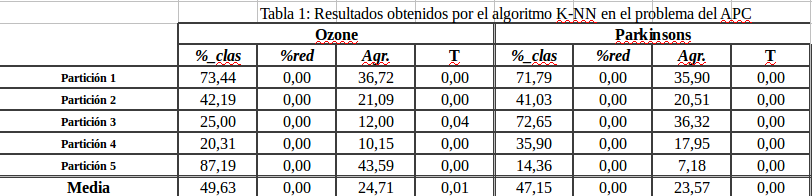
\includegraphics[width=14cm]{./K-NN.png}
	\end{center}
\end{figure}

\begin{figure}[htb]
	\begin{center}
		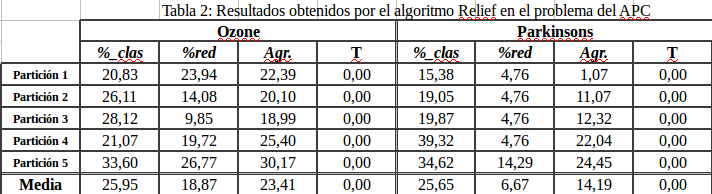
\includegraphics[width=14cm]{./Relief.png}
	\end{center}
\end{figure}

\begin{figure}[htb]
	\begin{center}
		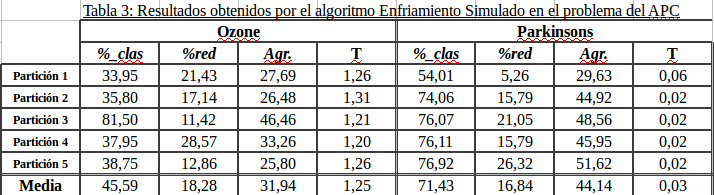
\includegraphics[width=14cm]{./ES.png}
	\end{center}
\end{figure}
\newpage
\begin{figure}[htb]
	\begin{center}
		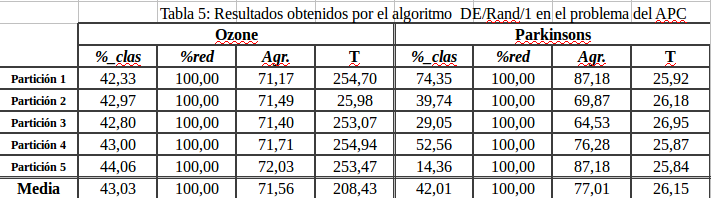
\includegraphics[width=14cm]{./ILS.png}
	\end{center}
\end{figure}

\begin{figure}[htb]
	\begin{center}
		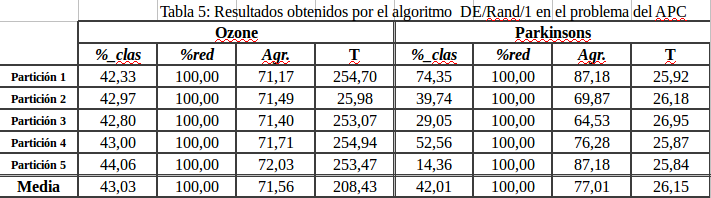
\includegraphics[width=14cm]{./DE_Rand.png}
	\end{center}
\end{figure}

\begin{figure}[htb]
	\begin{center}
		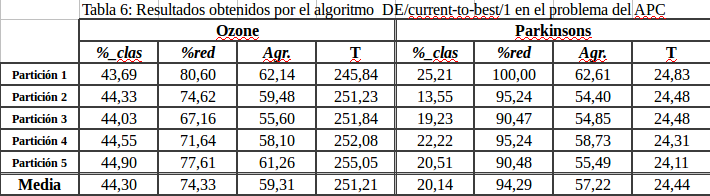
\includegraphics[width=14cm]{./DE_best.png}
	\end{center}
\end{figure}

\newpage

\begin{figure}[htb]
	\begin{center}
		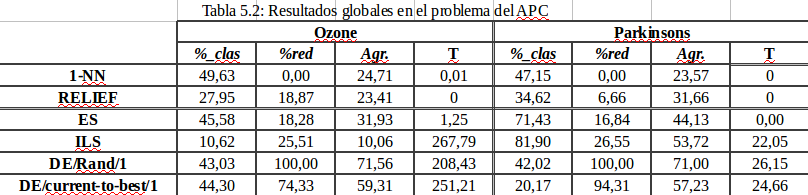
\includegraphics[width=12cm]{./Total.png}
	\end{center}
\end{figure}


Ya que tenemos todos los datos recogidos, antes de nada quiero comentar que los tiempos obtenidos han sido obtenidos aplicando optimización en tiempo de compilación, de nivel -O2. La ejecución total del programa, incluyendo la ejecución de todos los algoritmos para todos los conjuntos de datos, ha tomado un total de 3739,017 segundos, es decir 1 hora y 2 minutos.

Según los datos recogidos en la tabla de medias podemos ver que los mejores resultados para los conjuntos de datos que tenemos los conseguimos con los algoritmos basados en poblaciones. El algoritmo de \textit{Evolución Differencial} con cruce y mutación aleatoria ha obtenido los mejores resultados.

Comparando los algoritmos, podemos ver como K-NN y Relief obtienen unos peores resultados comparandolos con los algoritmos de Evolución Diferencial, ES, e ILS. A mi parecer, me resultan extraños los resultados obtenidos por los algoritmos K-NN, Relief y ES. Es posible que en algún paso de mi immplementación hay algo que no es correcto o algo así. De todos modos los buenos resultados de Evolución Diferencial si son más coherentes.
\end{document}


